\documentclass[../uilmath.tex]{subfiles}
\graphicspath{{\subfix{../figures/}}}
\begin{document}
\chapter{Statistics}
\section*{Problems}
\begin{enumerate}[label=\bfseries\arabic*.]
    \item %% Problem 1
    A box contains 5 green balls, 4 blue balls, and 3 red balls. Two balls are randomly selected, one at a time, without replacement. What is the probability that both are blue?

    \item %% Problem 2
    If two dice are rolled at one time, what is the probability that both dice show a prime number?

    \item %% Problem 3
    OVer the last few years, the length of Randy's drives at the local driving range follows a normal distribution with a mean of 
    225 yards and a standard deviation of 6 yards. Approximately what percentage of his drives are between 219 yards and 231 yards? (nearest whole number)

    \item %% Problem 4
    A fair die is rolled four times. What is the probability of getting an even number, a prime number, a Fibonacci number, and a perfect number, in that order?

    \item %% Problem 5
    Mel is throwing darts at a circular target with a diameter of 24. On the raget are two concentric circles with diameters 8 and 16. A dart landing in the small circle earns 10 points.
    A dart landing inside the circle with a diameter of 16, but outside the small circle earns 6 points. A dart landing on the target outside of the two concentric circles earns 2 points.
    Find the expected value of the points earned on any randomly selected toss that lands on the target. (nearest tenth)


    Use the table below for problems 6 and 7. Karen owns the Kwik Stop in Sundown. She believes that the number of water bottles sold each day 
    varies with the temperature. She made a table of the high temperature and the number of water bottles sold on the 15th day of the month, for the months of April through September.
    \begin{center}
        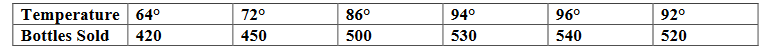
\includegraphics[width=0.8\textwidth]{2021SAC35.PNG}
    \end{center}
    \item %% Problem 6
    Find the sum of the mean, median, and range for the number of water bottles sold on these six days.

    \item %% Problem 7
    Use the data from the table to create an appropriate mathematical model and predict the high temperature on a day that Karen sold 354 water bottles. (nearest whole number)

    \item %% Problem 8
    The preferred swimming pool temperature of adult females follows a normal distribution with a mean of 82$\degree$ F with a standard deviation of $3\degree$ F. Find the probability that a random selected adult female 
    will prefer a temperature between $26\degree$ C and $29\degree$ C. (nearest thousandth)

    \item %% Problem 9
    A researcher took a random sample of 1,000 teenage males in order to estimate the mean number hours of sleep a typical 
    teenage boy gets each night. A 90\% confidence interval would be \blank than a 98\% confidence interval and would involve 
    \blank risk of being incorrect.

    \item %% Problem 10
    A one-stample $t$ statistic from a sample of 40 observations for the two-sided test of 
    \begin{center}
        $H_0 = 26$ \qquad $H_a\neq 26$
    \end{center}
    has the value $t=-1.44$. Find the $p$-value for this test. (nearest thousandth)

    \item %% Problem 11
    When analyzing data, statisticians often report the five-number summary. Which of the following are included in the five-number summary?\\
    I. mean \quad II. standard deviation \quad III. median \quad IV. quartiles \quad V. maximum and minimum

    \item %% Problem 12
    A shipment of twenty refurbished computers contains four defective computers. In how many ways 
    can Rocket purchase five of these computers and get two defective ones?

    \item %% Problem 13
    James has 6 calculus books and 8 physics books on his bookshelf at home. How many arrangements are possible if he keeps the calculus books together and the physics books together?


    \begin{center}
        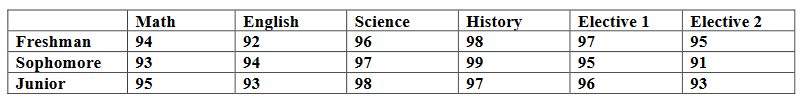
\includegraphics[width=0.8\textwidth]{2022SAC50.PNG}
    \end{center}
    Use the table above for problems 14 and 15.\\
    The table shows the grades for Carolyn her first three years at HPHS.
    \item %% Problem 14
    What is Carolyn's cumulative average after three years of school? (nearest hundredth)

    \item %% Problem 15
    If Carolyn needs to have a cumulative average of 95.45 or higher to graduate in the top 10, what is the minimum 
    average required during her senior year to meet this goal? She plans to take 6 courses her senior year. (nearest hundredth)

    \item %% Problem 16
    Suppose the distribution of the heights of adult males in Nevada is approximately normal with a mean height of 70 inches 
    and a standard deviation of 2.7 inches. A height of 72 inches corresponds to what percentile in the distribution?

    \begin{center}
        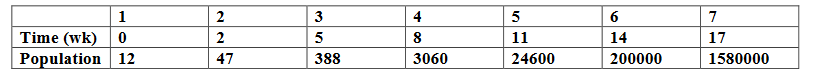
\includegraphics[width=0.8\textwidth]{2022SAC55.PNG}
    \end{center}
    Use the table above for problems 17 and 18.\\
    Sam was doing research for his master's thesis at Harvard. He estimated the population 
    of an isolated group of flies at seven different times. He started at $t=0$ with 12 flies. He finished at $t=17$ weeks with 1,580,000 flies.
    \item %% Problem 17
    Sam entered the data into a list he called $L_1$ and the populations into a list he called $L_2$ on his computer. Which of the following transformation equations will linearize the data?
        
    $\textbf{(A) } (L_1,(L_2)^3) \qquad \textbf{(B) } ((L_1)^3,L_2) \qquad \textbf{(C) } (\log(L_1),L_2) \qquad \textbf{(D) } (L_1,\log(L_2)) \qquad \textbf{(E) } (\log(L_1),\log(L_2))$

    \item %% Problem 18
    Sam was successful in using one of the transformations listed in problem 17 to calculate a regression equation that fit the data. Use this equation 
    to predict how many days after $t=0$ that the population reaches 100,000 flies. (nearest tenth)

    \item %% Problem 19
    Four-hundred students at Texas Tech were randomly selected and asked if they had worked out at the Recreation Center by using a treadmill or an elliptical trainer the past week.
    The results showed that 75 had worked out on both, 190 had worked out on a treadmill, and 260 had worked out on an elliptical trainer. How many of the 400 students 
    stampled had not worked out on either training device the previous week?

    \item %% Problem 20
    Amarillo Slim was playing five card poker. He had a full house, but lost to the dealer who had a royal flush. This is where a player 
    has the ten, jack, queen, king and ace of the same suit. Slim thought the dealer was cheating because the probability of being dealt a royal flush from a standard deck of 52 cards 
    is only $\blank$. (9 decimal places)

    \item %% Problem 21
    Assume that Luka Doncic makes 35.3\% of his 3-point shots regardless of the opponent or where the game is being played. He is 
    unaffected by previous attempts. If he attempts ten 3-points shots in a game, what is the probability that he makes 4, 5, or 6 of the shots? (nearest thousandth)

    \item %% Problem 22
    A survey asked a random sample of 500 U.S. teenagers whether music from the 1970s is superior to music from the 2020s.
    Of the sample, 312 responded with ``yes''. Construct a 95\% confidence interval for the proportion of U.S. teenagers who would say 
    ``yes'' if asked this question.

    \item %% Problem 23
    The average lifetime of battery packs for the Williams Electric vehicle was 4.9 years in 2004. In 2012, they introduced 
    a new battery pack that they believed would last longer. A simple random sample of 50 of the 2012 vehicles with the new battery 
    packs was selected. The mean lifetime of the battery packs turned out to be 5.1 years with a standard deviation of 0.86 years. An appropriate
    test was performed and the resulting $P$-value was $\blank$. (nearest thousandth)

    \item %% Problem 24
    Andrew has 12 marbles that are identical in size, but vary in color. Three are red, four are blue and five are green.
    If he wishes to place them in a straight line on a table, how many distinct arrangements can be made?

    \item %% Problem 25
    The ``on base percentage'' for Maury Wills of the Portland Beavers is 0.355. If he has 10 at bats in a doubleheader 
    against the Billings Broncos, what is the probability that he will safely get on base exactly 4 times. (Nearest hundredth)


    \begin{center}
        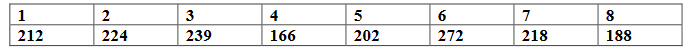
\includegraphics[width=0.8\textwidth]{2023SAC51.PNG}
    \end{center}
    Brent loves to bowl. The table above shows the scores from the eight games he bowled on Friday night at 
    Salado Lanes. Use this table for problems 26 and 27.
    \item %% Problem 26
    Find the positive difference between Brent's mean score and median score.

    \item %% Problem 27
    How many of his scores are classified as outliers?


    \begin{center}
        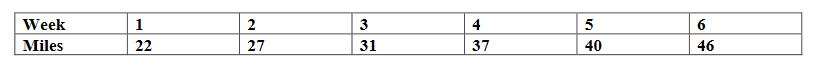
\includegraphics[width=0.8\textwidth]{2023SAC54.PNG}
    \end{center}
    Use the table above for problems 28 and 29.
    \item %% Problem 28
    Carmen began her 10-week buildup for cross country in June. She ran at 7-minute pace over hilly terrain and gradually increased her mileage each week. The table above shows her mileage 
    total for each of the first six weeks of her buildup. When she plotted her data, she believed a linear model fit her data pretty well. Use a linear model to predict her mileage for week 10. (nearest tenth)

    \item %% Problem 29
    If she actually ran 58 miles in week 8, what is the residual for week 8? (nearest hundredth)

    \item %% Problem 30
    Four hundred seniors are enrolled in the Patton Springs Stem Academy. Two hundred sixteen are taking Calculus, one hundred eighty-four are taking Statistics, 
    and one hundred forty-eight are taking Physics. Thirty-six are taking Statistics and Calculus, but not Physics. Sixty-four are taking Calculus and Physics, but not Statistics.
    Twenty-two are taking Statistics and Physics, but not Calculus. Sixty-two are not taking any of these three classes. How many seniors are taking all three of these classes?

    \item %% Problem 31
    There are so many students applying to attend the Patton Springs Stem Academy that a math readiness test is given to all applicants and the scores 
    on these tests are used as part of the admission process. The mean score on math readiness test is 856 with a standard deviation of 48. If Kyle scored 915 on the math readiness test, what percentile does that place him at? (nearest tenth)

    \item %% Problem 32
    Assume that the mean distance for the men's shot in Diamond League competition is 65 ft 2 in with a standard deviation of 4 ft 1 in. For women, 
    assume the mean distance is 58 ft 3 in with a standard deviation of 3 ft 11 in. If Ryan's best is 77 ft and 3.75 in and Valerie's best is 69 ft 8 in, who had a better performance 
    based on $z$-scores? Ryan's performance was slightly better because his $z$-score minus Valerie's $z$-score $=\blank$. (nearest thousandth)


    A large Supermarket chain requires that no more than 10\% of apples they receive have defects. When a recent shipment came in, inspectors took a random sample of 400 apples and they determined that 50 of the apples 
    had defects. The data was given to a highly paid analyst. She performed an appropriate test at the $\alpha = 0.05$ level and made a recommendation.
    \item %% Problem 33
    The appropriate test was the \blank Test.

    \item %% Problem 34
    Based on a $P$-value of \blank (nearest thousandth), she recommended the shipment be rejected.

    \item %% Problem 35
    Andrew has 12 marbles that are identical in size, but vary in color. Six are red, four are blue and two are green.
    If he wishes to place them in a straight line on a table, how many distinct arrangements can be made?

    \item %% Problem 36
    The ``on base percentage'' for Bobby Richardson of the Yankees is 0.328. If he has 9 at bats in a doubleheader 
    against the Dodgers, what is the probability that he will safely get on base exactly 5 times? (nearest hundredth)


    Use the following table for problems 37 and 38.
    \begin{center}
        
\includegraphics[width=0.8\textwidth]{2024SAC53.PNG}
    \end{center}
    Joe tries to exercise every day at the gym. He runs, lifts weights, and uses a Stair Master.
    Last week, he recorded the time he spent at the gym as shown in the table above.
    \item %% Problem 37
    Find the positive difference between the mean and the median of the data.

    \item %% Problem 38
    A modified box plot shows that there are \blank outliers.


    Use the following table for problems 39 and 40.
    \begin{center}
        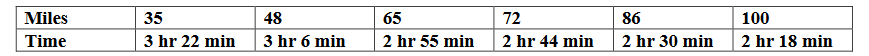
\includegraphics[width=0.8\textwidth]{2024SAC55.PNG}
    \end{center}
    Six men of similar abilities spent 6 months preparing for the Houston marathon. Their average weekly mileage and their times for the race are shown in the table above.
    Coach Salazar plotted the data in the table and decided that a linear relationship existed between the average weekly mileages of his runners and their times at the Houston Marathon.
    He used statistical software to generate a least squares regression line (LSRL).
    \item %% Problem 39
    The LSRL predicts that for each increase of one mile in a runner's weekly mileage, there is a corresponding decrease of \blank seconds in their marathon time. (nearest whole number)

    \item %% Problem 40
    According to the model, what should a runner's average weekly mileage be in order to run a marathon in 2 hr 10 min? (nearest whole number)

    \item %% Problem 41
    In a random sample of 32 adult male wild turkeys found in Hemphill County, the average weight was 20 pounds with a standard deviation of 2 pounds.
    Construct a 96\% confidence interval for the mean weight of adult male turkeys found in Hemphill County. (nearest hundredth)

    \item %% Problem 42
    At Aberdeen High School, 58\% of the students are girls and 42\% are boys. Suppose that 72\% of the girls select soccer as their 
    sport compared to 36\% for the boys. If a randomly selected student selects soccer as his/her favorite sport, what is the probability that the student is a girl? (nearest hundredth)

    
    For problems 43 and 44, assume that the average drive for a 74-year-old male golfer is 226 yards with a standard deviation of 12 yards.
    \item %% Problem 43
    If Randy is 74 years old and his average drive is 237 yards, what percentile does that place him at among 74-year-old golfers?

    \item %% Problem 44
    If a 74-year-old male golfer wanted to be at the 96th percentile, what average drive is required? (nearest whole number)

    \item %% Problem 45
    Iva Gottadele bought an autographed bat on Ebay for \$28.00. She estimates that there is a 35\% probability
    that she can resell it for \$36.00 and a 65\% probability that she will only be able to resell it for \$23.00.
    What is the mathematical expectation of this deal?

    \item %% Problem 46
    The following test scores are listed in order from least to greatest: $75,x,85,y,88,91,z$.
    Find the mean of the scores if the median score is 86, the mode score is 75, and the range is 20.

    \item %% Problem 47
    Coach Barton has 10 students on his math team. He wants to arrange them into practice teams 
    of 3 or 4 students. How many practice teams can he make?

    \item %% Problem 48
    The odds of losing an event is $\frac{a}{b}$. The probability of winning the event is:

    \item %% Problem 49
    If the probability that a student in a Statistics class studies for an exam is 75\%, and the probability that a student who 
    studies passes the test is 90\%, then the probability that a student both studies and passes the test is: 

    \item %% Problem 50
    Betty Wheel spins the Wheel of Fun. The wheel consists of eight congruent sectors as shown. What is the mathematical expectation on any one spin?
    \begin{center}
        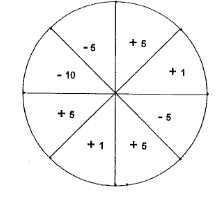
\includegraphics[width=0.4\textwidth]{2008B22.PNG}
    \end{center}

    \item %% Problem 51
    The probability of scoring less than 200 on this test is 75\%. What are the odds of a student scoring greater than or equal to 200 on this test?

    \item %% Problem 52
    Berry Kold Creamery has four flavors of ice cream: vanilla, pistachio, black walnut, and strawberry. The daily sundae has three scoops of ice cream. How many variations of sundaes are there?

    \item %% Problem 53
    Fifty-Fifty High School has five male teachers and five female teachers. How many ways are there to form a committee of three female teachers and two male teachers?

    \item %% Problem 54
    Six boys and twelve girls are in the senior class. Half the boys and 25\% of the girls wear glasses. What is the probability that a student chosen randomly is a boy, wears glasses, or both?

    \item %% Problem 55
    Let $E=\{0,2,4,6,8\}$. Two elements of set $E$ are selected at random without replacement.
    What is the probability that the mean of the two numbers selected is an odd number?

    \item %% Problem 56
    Seymore Endelite randomly selects two socks from his drawer to wear to school. The socks are identical except for their color 
    and are not paired up. He has 8 blue socks, 6 black socks, and 4 white socks. What is the probability that he selects two black socks? (nearest percent)

    \item %% Problem 57
    Lotta Dough has a bag that contains one \$100 bill, two \$20 bills, three \$10 bills, four \$5 bills, and five \$1 bills. The odds of her pulling out a \$10 bill is 25\%. How many 
    \$10 bills would have to be added to the bag to change the odds to 50\%?

    \item %% Problem 58
    Find the ratio of the median to the mean of the following list of numbers:
    \begin{center}
        2, 3, 5, 2, 4, 3, 2, 0, 5, 3, 5, 2
    \end{center}

    \item %% Problem 59
    Betty Luzes rolls a fair die 4 times. What is the mathematical expectation of the sum of the outcomes of the 4 rolls?

    \item %% Problem 60
    Five married couples attend the square dance planning meeting. How many committees of four people can be chosen if no committee is to include a husband-and-wife pair?

    \item %% Problem 61
    A regular deck of 52 cards is shuffled and the top five cards are dealt face up. What is the probability, nearest $\frac{1}{1000}$\%, that all 5 cards are face cards (Jacks, Queens, Kings)?

    \item %% Problem 62
    Ronald Tuwin is playing a special dice game. He rolls two dice. If he rolls a double $(1-1, 2-2,3-3$, etc.) he gets 20 points.
    If he does not roll a double and the sum of the dice is a prime number he gets 10 points. If he does not roll a double and the number is not a prime, he loses 5 points.
    What is the mathematical expression on any one roll?

    \item %% Problem 63
    Betty Cheetz flips a fair coin and rolls a fair six-sided die. What are the odds that she will get a head and a prime number?

    \item %% Problem 64
    Let $L=\{2,1,3,4,7,11\}$. Two elements of set $L$ are selected at random without replacement.
    What is the probability that the median of the two numbers selected is a whole number?

    \item %% Problem 65
    How many different ways can you select 5 bills from a cash box containing \$1, \$2, \$5, \$10, \$20, \$50, and \$100 bills?

    \item %% Problem 66
    A bag contains yellow golf balls and orange golf balls. The probability of selecting a yellow ball is $\frac{2}{5}$. If 20 yellow balls 
    are added to the bag, the probability of selecting a yellow ball becomes $\frac{4}{7}$. How many orange balls are in the bag?

    \item %% Problem 67
    The Buddy System motorcycle testing company is testing a motorcycle with a side car. They hire 4 cyclists 
    to do the testing in pairs. How many arrangements of driver and rider are possible?

    \item %% Problem 68
    A box contains four rods whose lengths are 2'', 3'', 5'', and 7''. How many different triangles can be made using only three rods at a time.

    \item %% Problem 69
    A box contains circular poker chips that are congruent in shape but not color. There are red ones, white ones, and blue ones.
    Drew Goode randomly draws out a chip. He gets 5 points if it is a blue one, 1 point for a white one, and he loses 3 points for a red one.
    The probability of drawing out a red one is 25\%, a blue one is 6\%, and a white one is 15\%. What is his mathematical expectation on any one draw?

    \item %% Problem 70
    How many different letter arrangements can be made by rearranging the letters in the word `LETTER'?

    \item %% Problem 71
    Willie Lawkit can't remember the combination to the padlock shown. He knows that the first number is greater than 30, 
    the second number is a positive Fibonacci number, and the third number is a factor of 30. How many combinations can he try to open the lock?
    \begin{center}
        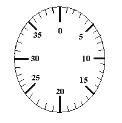
\includegraphics[width=0.3\textwidth]{2010A45.PNG}
    \end{center}

    \item %% Problem 72
    Coach Winters has 4 seniors, 5 juniors, 3 sophomores, and 4 freshman on her math team. How many ways can she form practice groups of 
    four members consisting of one member from each of the grade levels?

    \item %% Problem 73
    Romeo, Juliet, and three classmates are randomly assigned seats in a row of five chairs. What is the probability that Romeo and Juliet will be seated next to each other?

    \item %% Problem 74
    Ronald Bones found a die with 6 blank faces on it. He painted the numbers $1,1,2,3,5,\& 8$, one number per face, on the die.
    He created a game such that he gets 10 points if he rolls a composite number, he gets 5 points if he rolls a prime number, and he loses 
    7 points if he rolls a unit. What would the mathematical expectation be for any given roll?

    \item %% Problem 75
    Two distinct numbers are selected randomly from the set $\{2,1,3,4,7,11\}$. What is the probability that their sum is an odd number?

    \item %% Problem 76
    Coach Fuhrmann has 8 boys and 6 girls in his math and science club. He needs to send a delegation to a UIL planning conference. 
    How many possible delegations can he send if each delegation must contain exactly 2 boys and exactly 2 girls?

    \item %% Problem 77
    Willie Bettit has 5 plain red poker chips, 3 plain white poker chips, and 2 plain blue poker chips. How many ways can he line all of them up in a row?

    \item %% Problem 78
    How many 5 digit numbers can be made using the digits $1,2,3,4 \& 5$ where the digits in the tens place and the hundreds place must be a prime number. Each digit can only be used once in a number.

    \item %% Problem 79
    The Cowboys and the Texans will play twice this season. The Cowboys are twice as likely to win any game as the Texans. What is the probability that they will each win one of the two games?

    \item %% Problem 80
    P-Q-R is the combination needed to open the safe with the combination dial shown below. How many distinct combinations exist if $P$ is a triangular number, $Q$ is a square number 
    greater than 0, $R$ is a pentagonal number.
    \begin{center}
        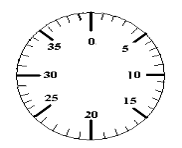
\includegraphics[width=0.3\textwidth]{2018A26.PNG}
    \end{center}

    \item %% Problem 81
    Roland Bones rolls a pair of dice. What are the odds that the sum of top faces he rolls is a $7$ or an $11$?

    \item %% Problem 82
    Arnie has a bag with 3 white golf balls and 2 yellow golf balls. Jack has a bag with 4 yellow golf balls and 2 white golf balls.
    Tiger picks a bag and a ball at random. The probability that the ball will be white is: (nearest whole percent)

    \item %% Problem 83
    Twenty-five seniors took the state math test last year. Fifteen of them were boys and ten were girls. All of them had an equal chance to win one of the top three medals. What was the probability that one girl and two boys won one of the top three medals? (nearest whole percent)

    \item %% Problem 84
    If the probability that a student in a Statistics class studies for an exam is 70\%, and the probability that a student who studies passes the test is 85\%, then the probability that a student both studies and passes the test is: (nearest whole percent)

    \item %% Problem 85
    In how many ways can the letters of the word `DIVIDE' be arranged in such a way that the vowels always come together?

    \item % 86
    Find the average of the arithmetic mean, the median, and the mode of these quiz grades: 75, 95, 75, 100, 95, 80, 75, \& 70. (nearest whole number)

    \item %% 87
    At a company, ten employees and ten interns line up to visit the CEO in ten randomly selected pairs. If each pair of employees 
    receives a copper ring, each pair of interns receives a brass ring, and each employee-intern pair receives a silver ring, what is the probability that the number of copper rings 
    received equals the number of brass rings received?

    \item %% 88
    In a triple play game, Willie When performs three tasks. He flips a quarter, and success would be heads. He rolls a single die, and success would be a six. He picks a card from a standard 
    deck of cards, and success would be picking a heart. If any of these tasks are successful, He will win the game. What is the probability he will win? (nearest whole percent)

    \item % 89
    If two dice are tossed, what is the probability that the sum of the faces is a prime number?

    \item % 90
    The Blow Upp balloon company package 6 balloons per pack. The company has red, blue, white, pink, yellow,
    green, and magenta colored balloons. How many different packs of 6 balloons can they package?

    \item % 91
    14 out of 17 Millersviewites have spouses. 4 out of 6 Millersviewites own at least 3 acres and a travel trailer. What is the probability
    that a Millersviewite has a travel trailer given that a Millersviewite has a spouse? (nearest whole percent)

    \item % 92
    Anthony and Chuck take three number sense tests. Anthony is twice as likely to s core higher than Chuck. What are the odds that Anthony scores higher on all three tests? Due to an unknown tiebreaker, there are no ties.

    \item % 93
    Thirty seniors took the state math test last year. Twenty-two of them were boys and eight were girls. All of them had an equal chance to win one 
    of the top three medals. What was the probability that two girls and one boy won one of the top three medals? (nearest whole percent)

    \item % 94
    A box of golf balls contains 6 white ones, 4 pink ones, and 2 blue ones. Three balls are randomly drawn from the box, without replacement.
    What are the odds that they are all the same color?

    \item % 95
    Betty Chuzrite selects one letter from each of the sets $\{a,c,u,t,e\}$ and $\{o,t,u,s,e\}$. What is the probability she selects one vowel? (nearest whole percent)

    \item % 96
    Betty Chuzrite selects one letter from each of the sets $\{a,c,u,t,e\}$ and $\{o,t,u,s,e\}$. What is the probability she selects at least one vowel? (nearest whole percent) 

    \item % 97
    How many distinct 4-letter code words can be made from the letters in the word ALGEBRA?

    \item % 98
    Les Avridge had quiz grades of $75,83,66,90,83,50,65$, and $83$. The average of the arithmetic mean, median, 
    mode, and range of his quiz grades is? (nearest whole number)

    \item % 99
    For the final exam in calculus, Mrs. Wilcox gave her class a list of 18 study problems. Of these, 10 will be on the exam. If Emmy knows how to correctly solve 16 of these,
    find the probability that she will correctly solve all 10 problems on the final exam. (nearest thousandth)

    \begin{center}
        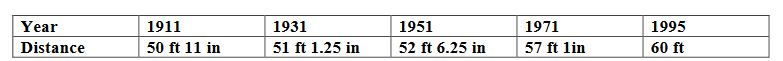
\includegraphics[width=0.7\textwidth]{2023D53.PNG}
    \end{center}
    The progression of the world record in the men's triple jump is shown in the table above. Use this table for problems 100 and 101.
    \item % 100
    Professor Stat instructed his students to find the LSRL for the data. The linear regression model overestimates the true value of the 1951 distance by \blank . (nearest hundredth)

    \item % 101
    Use the LSRL for the data and predict what the world record should be in 2022. (nearest inch)

    \item % 102
    Assume the mean hang time of a punt for all NFL punters over the 2022 season was 4.40 seconds with a standard deviation of 0.25 seconds. 
    If Jordan Stout had a mean hang time of 4.82 seconds for the 2022 season, what percentile did that place him at?

    \item % 103
    Consider a random variable $X$ that is normally distributed with a mean of 75 and a standard deviation of 16.
    The approximate interquartile range for this distribution is \blank . (nearest tenth)

    \item % 104
    A random sample of 500 Texas high school students is used to estimate the proportion of Texas high school students who participate in UIL academics.
    What is the maximum margin of error if a 96 percent confidence interval is to be constructed? (nearest thousandth)

    \begin{center}
        
\includegraphics[width=0.7\textwidth]{2023D58.PNG}
    \end{center}
    \item % 105
    A random sample of 360 high school seniors in the Texas Panhandle were asked which university they hoped to attend.
    Students were asked to choose between Texas, A\&M, Tech, and TCU. The results are in the able above. Researchers had expected a ratio of $3:3:4:2$ for their choices.
    An appropriate test at the $\alpha = 0.05$ level was performed to see if the observed values differ from what was expected. Based on a $P$-value of \blank, researchers concluded that 
    there was insufficient evidence to show that student choices differ from what was expected.

    \item % 106
    Ninety-five percent of the Olympic athletes who have been using steroids will test positive using a new test just developed. Ninety-eight percent of Olympic athletes who have not been using steroids will test negative 
    using the new test. If ten percent of Olympiad athletes have been using steroids, what percent of Olympic athletes will test positive using the new test? (nearest tenth)

    \item % 107
    In the Fort Bend school district, 16 out of 88 randomly selected high school seniors plan to study computer science in college, while 21 out of 72 juniors plan to study computer science in college.
    A 96\% confidence interval for the difference between the proportion of high school seniors who plan to study computer science in college and the proportion of high school juniors who plan to study computer science is to be calculated.
    What is the standard error of difference? (nearest ten-thousandth)

    \item % 108
    Two numbers are selected from the set $E=\{1,2,3,4,5\}$ at random. What is the probability that the product of the two numbers is less than 10?

    \item % 109
    Computer World in Big Timber, Montana currently has 20 computers in stock. Fifteen have 16 GB RAM and five have 8 GB RAM. If Rancher Rob randomly selects four computers to purchase, what is the probability that at least two of the computers have 16 GB RAM? (nearest thousandth)

    \item % 110
    The Lick'em Slow lollipop company package 5 lollipops per pack. The company has chocolate, raspberry, coconut, grape, lime, and licorace lollipops. How many different packs of 5 lollipops can they package?

    \item % 111
    Nicole Taas is going to flip a coin three times and record the results. What is the probability she gets at least one head? (nearest wholer percent)

    \item % 112
    Nicole Taas is going to flip a coin three times and record the results. What are the odds against her getting exactly two heads?

    \item % 113
    N.A. Hurry stops at a convenience store. The probability that she buys a loaf of bread is $60\%$, the probability she buys a gallon of milk is $50\%$, and the probability she buys both bread and milk is $30\%$. What is 
    the probability she will buy either bread or milk or both?

    \item % 114
    Nicole Taas is going to flip a coin three times and record the results. What is the probability she gets at least two tails given that the first flip was a tail. (nearest whole percent)

    \item % 115
    How many distinct 4-letter code words can be made from the letters in the words ``PIZZA PIE'' if the first letter must be a vowel and the second letter must be a consonant?

    \item % 116
    
\end{enumerate}
\section*{Solutions}
\begin{enumerate}[label=\bfseries\arabic*.]
    \item %% Problem 1
    $\frac{1}{11}$

    \item %% Problem 2
    25\%

    \item %% Problem 3
    68\% 

    \item %% Problem 4
    $\frac{1}{36}$

    \item %% Problem 5
    4.2

    \item %% Problem 6
    $1123.\overline{3}$

    \item %% Problem 7
    $46\degree$

    \item %% Problem 8
    0.625

    \item %% Problem 9
    narrower, a greater 

    \item %% Problem 10
    0.158

    \item %% Problem 11
    III, IV, V 

    \item %% Problem 12
    3360

    \item %% Problem 13
    58,060,800

    \item %% Problem 14
    95.17

    \item %% Problem 15
    96.30

    \item %% Problem 16
    77th

    \item %% Problem 17
    D 

    \item %% Problem 18
    91.1 days 

    \item %% Problem 19
    25

    \item %% Problem 20
    .000001539

    \item %% Problem 21
    0.467 

    \item %% Problem 22
    $(.5815, .6665)$

    \item %% Problem 23
    0.053

    \item %% Problem 24
    27,720

    \item %% Problem 25
    0.24

    \item %% Problem 26
    0.125

    \item %% Problem 27
    0

    \item %% Problem 28
    64.5 mi 

    \item %% Problem 29
    2.95 mi 

    \item %% Problem 30
    44

    \item %% Problem 31
    89th 

    \item %% Problem 32
    0.060

    \item %% Problem 33
    One Sample $z$ Test for a Proportion 

    \item %% Problem 34
    0.048

    \item %% Problem 35
    13,860

    \item %% Problem 36
    0.10

    \item %% Problem 37
    3 min

    \item %% Problem 38
    0

    \item %% Problem 39
    59

    \item %% Problem 40
    108 mi 

    \item %% Problem 41
    ${19.24, 20.76}$

    \item %% Problem 42
    0.73

    \item %% Problem 43
    82nd

    \item %% Problem 44
    247 yd 

    \item %% Problem 45
    \$27.55

    \item %% Problem 46
    85

    \item %% Problem 47
    330 

    \item %% Problem 48
    $\frac{b}{a+b}$

    \item %% Problem 49
    67.5\%

    \item %% Problem 50
    -.375

    \item %% Problem 51
    1 to 3 

    \item %% Problem 52
    20

    \item %% Problem 53
    100

    \item %% Problem 54
    50\%

    \item %% Problem 55
    60\%

    \item %% Problem 56
    10\%

    \item %% Problem 57
    3

    \item %% Problem 58
    1:1 

    \item %% Problem 59
    14

    \item %% Problem 60
    80

    \item %% Problem 61
    $\frac{3}{100}$\% 

    \item %% Problem 62
    5 points 

    \item %% Problem 63
    $\frac{1}{3}$

    \item %% Problem 64
    $46\frac{2}{3}$\%

    \item %% Problem 65
    462

    \item %% Problem 66
    30

    \item %% Problem 67
    12

    \item %% Problem 68
    1

    \item %% Problem 69
    2.4

    \item %% Problem 70
    180

    \item %% Problem 71
    576

    \item %% Problem 72
    240

    \item %% Problem 73
    40\%

    \item %% Problem 74
    $-2\frac{1}{3}$ pts 

    \item %% Problem 75
    $46\frac{2}{3}$\% 

    \item %% Problem 76
    1,680 

    \item %% Problem 77
    3,628,800

    \item %% Problem 78
    48 

    \item %% Problem 79
    $66\frac{2}{3}$\%

    \item %% Problem 80
    240

    \item %% Problem 81
    $\frac{2}{7}$

    \item %% Problem 82
    $47\%$

    \item %% Problem 83
    $46\%$

    \item %% Problem 84
    $60\%$

    \item %% Problem 85
    36 

    \item % 86
    79

    \item %% 87
    1

    \item % 88
    69\%

    \item % 89
    $\frac{5}{12}$

    \item % 90
    924

    \item % 91
    81\%

    \item % 92
    $\frac{8}{19}$

    \item % 93
    15\%

    \item % 94
    12\%

    \item % 95
    48\%

    \item % 96
    84\%

    \item % 97
    480

    \item % 98
    69

    \item % 99
    0.183 

    \item %100
    1.71 ft 

    \item % 101
    62 ft 6 in 

    \item % 102
    95th

    \item % 103
    21.6

    \item % 104
    0.046

    \item % 105
    0.346

    \item % 106
    11.3\%

    \item % 107
    0.0675

    \item % 108
    .6

    \item % 109
    0.968

    \item % 110
    252

    \item % 111
    88\%

    \item % 112
    $5:3$

    \item % 113
    $80\%$

    \item % 114
    $75\%$

    \item % 115
    98

    \item % 116
    
\end{enumerate}

\end{document}